% Created 2016-08-17 Wed 14:38
\documentclass[tikz]{standalone}

\usepackage[utf8]{inputenc}
\usepackage[T1]{fontenc}
\usepackage{helvet}
\usepackage{../../templates/msc}

\renewcommand{\familydefault}{\sfdefault}

\tikzset{
every picture/.style={
line width=1pt
}}

\usepackage{tikz}
\author{Holger Karl}
\date{\today}
\title{}

\usepackage{tikzsymbols}


\begin{document}
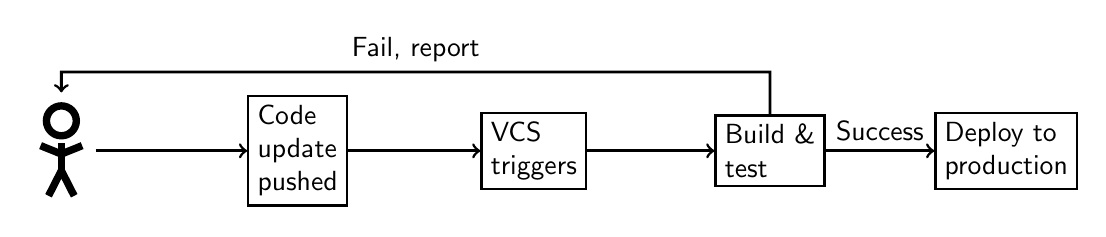
\begin{tikzpicture}[auto, xscale=3,
block/.style = {rectangle, draw=black, thick, align=left}]
  % \node [block]  at (0,1) (sender) {\textbf{Sender:} \\x = native data;\\px = pack(x);
  %   \\send(px);};
  % \node [block] at (2,3) (idl) {Data definition file};
  % \node [block] at (2,2) (idlcomp) {IDL compiler};
  % \node [block] at (1,1) (pack) {pack()}; 
  % \node [block] at (3,1) (unpack) {unpack()}; 
  % \node [block]  at (4,1) (receiver) {\textbf{Receiver:} \\px =  receive();\\x = unpack(px);
  %   \\//use native data in x };
  % %
  % \draw [->] (idl) -- (idlcomp); 
  % \draw [->] (idlcomp) -- (pack); 
  % \draw [->] (idlcomp) -- (unpack); 
  % \draw (-1,-1) -- (5,-1);
  % \draw [->] (sender) -- (0, -1); 
  % \draw [->] (4, -1) -- (receiver); 
  % \draw  [->] (sender.east) to [bend left=80] (pack.west) ; 
  % \draw  [->] (pack.west) to [bend left=45] (sender.east) ; 
  % \draw  [->] (receiver.west) to [bend left=45] (unpack.east) ; 
  % \draw  [->] (unpack.east) to [bend left=45] (receiver.west) ; 
  % \path (sender) edge [bend north ] node [right] {} (pack);

\node at (-1,0) (h)  {\Strichmaxerl[5]}; 
\node [block] at (0,0) (c)  {Code\\update\\pushed}; 
\node [block] at (1,0) (v)  {VCS\\triggers}; 
\node [block] at (2,0) (b)  {Build \&\\test}; 
\node [block] at (3,0) (p)  {Deploy to \\production}; 
\draw [->] (h) -- (c); 
\draw [->] (c) -- (v); 
\draw [->] (v) -- (b); 
\draw [->] (b) -- node [above] {Success} (p); 
\draw [->] (b) -- (2,1) --  node [above] {Fail, report} (-1,1) --(h); 

\end{tikzpicture}
\end{document}